%
% File ucca_parsing.tex
%

\documentclass[11pt]{article}
\usepackage{acl2016}
\usepackage{times}
\usepackage{url}
\usepackage{amsmath}
\usepackage{breqn}
\usepackage{latexsym}
\usepackage{pgfplotstable}
\usepackage[]{algorithm2e}
\usepackage{hhline}
\usepackage{multirow}
\usepackage{caption}
\usepackage{subcaption}
\usepackage{hyperref}
\usepackage{color}
\usepackage{lipsum,adjustbox}
\usepackage{tikz}
\usepackage{tikz-dependency}
\usetikzlibrary{shapes,fit,calc,er,positioning,intersections,decorations.shapes,mindmap,trees}
\tikzset{decorate sep/.style 2 args={decorate,decoration={shape backgrounds,shape=circle,
      shape size=#1,shape sep=#2}}}

\newcommand{\oa}[1]{\footnote{\color{red} #1}}
\newcommand{\daniel}[1]{\footnote{\color{blue} #1}}
\newcommand{\com}[1]{}
\newcommand{\secref}[1]{Section~\ref{#1}}
\newcommand{\figref}[1]{Figure~\ref{#1}}
\newcommand{\tabref}[1]{Table~\ref{#1}}
\DeclareMathOperator*{\argmin}{argmin}
\DeclareMathOperator*{\argmax}{argmax}
\SetKwRepeat{Do}{do}{while}

%\aclfinalcopy % Uncomment this line for the final submission
%\def\aclpaperid{***} %  Enter the acl Paper ID here

% To expand the titlebox for more authors, uncomment
% below and set accordingly.
% \addtolength\titlebox{.5in}    

\newcommand\BibTeX{B\textsc{ib}\TeX}


\title{Broad-Coverage Semantic Parsing: A Transition-Based Approach}
  %General Transition-Based Broad-Coverage Semantic Parsing

\author{Daniel Hershcovich \and Omri Abend \and Ari Rappoport \\
  Institute of Computer Science \\
  Hebrew University of Jerusalem \\
  {\tt \{danielh,oabend,arir\}@cs.huji.ac.il}
}

\date{}


\begin{document}
\maketitle

%%%%%%%%%%%%%%%%%%%%%%%%%%%%%%%%%%%%%%%%%%%%%%%%%%%%%%%%%%%%%%%
%%%%%%%%%%%%%%%%%     Abstract
%%%%%%%%%%%%%%%%%%%%%%%%%%%%%%%%%%%%%%%%%%%%%%%%%%%%%%%%%%%%%%%
\begin{abstract}

  The representation of many common semantic phenomena requires
  more formal expressivity than is commonly used for syntactic parsing.
  %Recent work has focused on broad-coverage semantic parsing into dependency
  %  (word to word) or abstract (i.e., not grounded in the sentence's
  %words and phrases) representations.
  Existing representations and parsers mostly support some of these structural
  properties, which we term ``Broad-coverage semantic structures'' (BSS), but not all. 
  The main contribution of this paper is in proposing two transition-based
  techniques for parsing into BSS:
  (1) applying conversion procedures to BSS, mapping them into related
  formalisms, and using existing state-of-the-art parsers on the converted
  representations; and (2) constructing a novel parser for the task.
  We obtain encouraging results, using the UCCA semantic representation, which
  supports BSS, as a testbed.
  
  %Instead, we advocate a constituency-based formulation of the
  %  task and define the Broad-coverage Constituency Semantic Parsing task
  %  using 
  %  We note that there are no existing methods for constituency DAG parsing,
  %  and propose two transition-based approaches to tackle it:
  %%  semantic parsing tasks, and suggest future directions for improvement.
  
  %We experiment with two types of semantic representations, obtaining
  %encouraging results.
  %Universal Conceptual Cognitive Annotation (UCCA) is a semantic grammatical scheme
  % that assigns 
  %a complete structure to natural language text. We present the first automatic
  % UCCA parser, 
  % a transition-based parser using a novel transition system. We compare the
  % results to baselines 
  % obtained by converting UCCA to CoNNL-X, and training syntactic parsers on the
  % converted dependency trees.
  
\end{abstract}



%%%%%%%%%%%%%%%%%%%%%%%%%%%%%%%%%%%%%%%%%%%%%%%%%%%%%%%%%%%%%%%
\section{Introduction}

In order to support a full range of semantic structures, the following
structural properties are needed. First, arguments and relations (semantic units, or simply
units) that are shared between predicates are effectively represented as multi-parented nodes,
yielding DAG, rather than tree structures. For instance, in the sentence
``After graduation, John moved to Paris'', ``John'' is an argument of both ``graduation''
and ``moved'', yielding a DAG rather than tree structure (\figref{fig:graduation}).
Second, semantic structures require non-terminal nodes for complex units.
While bi-lexical dependencies partially circumvent this restriction, by
representing complex units in terms of their heads, they fall short
when representing units that have no clear head.
Frequent examples of such constructions include
coordination structures (e.g., ``{\bf John and Mary} went home''; \figref{fig:home})
some multi-word expressions (e.g., ``The Haves and the {\bf Have Nots}''),
and prepositional phrases.
Third, semantic units may be discontiguous in the text. For instance, in ``John gave everything up'' (\figref{fig:gave}),
the phrasal verb ``gave ... up'' forms a single semantic unit.
We call the combination of these three properties
{\it Broad-coverage Semantic Structures} (BSS).

However, to our knowledge, no existing parser supports the combination of these criteria,
and the only semantically-annotated corpora that supports them is UCCA \cite{abend2013universal}.
Several other models either support some of these properties \cite{oepen2015semeval},
or take an alternative approach and avoid grounding semantic units
altogether (notably, AMR \cite{banarescu2013abstract}). We discuss related work in \secref{sec:related}.

In this work we are thus first in proposing techniques for parsing BSS.
We adopt a transition-based approach, which has recently produced some of the best
results in syntactic dependency parsing
\cite{dyer2015transition,ballesteros2015improved}, and has demonstrated
strong performance in a variety of other semantic and syntactic settings as well
\cite{maier2015discontinuous,ambati2015incremental,wang2015transition}.

We pursue two complementary parsing strategies.
First, we assess the ability of existing technology to tackle the task,
by developing conversion protocols between UCCA structures and two related formalisms:
dependency trees and discontinuous constituency trees.
As these formalisms are more restrictive than BSS, the conversion
is necessarily lossy. Nonetheless, we find that it is effective
in practice (\secref{sec:conversion_approach}).

Second, we present a novel transition-based constituency DAG parser
that supports discontinuous constituents, named
the \textsc{bss} parser (\secref{sec:direct_approach}).\oa{add one-two sentences
  about the novelty of parsing techniques}

%and tackle the constituency-based semantic parsing task.
%Constituency semantic representation differ from previous broad-coverage semantic parsing
%work in two ways.
%First, it does not impose the unique head assumption, imposed
%by bi-lexical dependencies, which is problematic for representing several
%frequent constructions that have no clear head.
%Second, it grounds the representation in the text,
%unlike more abstract approach such as AMR \cite{banarescu2013abstract},
%which allows for the use of strong and efficient parsing methods.

We use the English UCCA-annotated corpora \cite{abend2013universal} as a test
case\footnote{While the task is not specific to UCCA,
  to the best of our knowledge, UCCA's are the only
  semantically annotated corpora that support all criteria of BSS.},
and apply the parsing approaches both to in-domain and out-of-domain scenarios.
Results are encouraging, with nealy 70\% labeled F-score for the highest
scoring parser, and suggest concrete paths for further improvement.
%a small degradation with the transition to out-of-domain scenarios.
All converters, parsers and datasets will be made publicly available upon publication.

%A general parser for this setting must support the prediction of multiple parents,
%as well as of discontiguous constituents, both pervasive phenomena in semantic
%structures even in English (see \secref{sec:data}.
%Multiple parents show up frequently in the context of argument
%sharing, where a certain argument participates in several relations but is only mentioned once.
%Common examples are coordination structures
%(e.g., in ``John went home and took a shower'', ``John'' is an argument of both ``went'' and ``took'')
%or nominalizations (e.g., ``After graduation, John moved to London'', where ``John'' is an argument
%of both ``graduation'' and ``moved'').
%Discontiguous units are common even in syntactic structures in some languages (e.g., German, Bulgarian,
%Korean and many others \cite{kallmeyer2013data}), and can even be found in English, e.g., in reported
%speech: ``'The dog', John said, 'is back again''', and are even more pervasive in English semantic parses
%(see \secref{sec:data}).

%\oa{fix this}
%The contribution of this work is thus three-fold.
%First, we motivate and define the constituency broad-coverage semantic parsing task.
%Second, we create converters and study the ability of existing parsing technology
%for formally related settings to address the task, focusing on transition-based methods.
%Third, we present the \textsc{bcs} parser, novel both in being the first constituency DAG parser,
%as well as the first UCCA parser. 

%%%%%%%%%%%%%%%%%%%%%%%%%%%%%%%%%%%%%%%%%%%%%%%%%%%%%%%%%%%%%%%
\section{Background}\label{sec:related}

\begin{figure}
  \begin{subfigure}[t]{.5\textwidth}
  \centering
  \scalebox{.9}{
  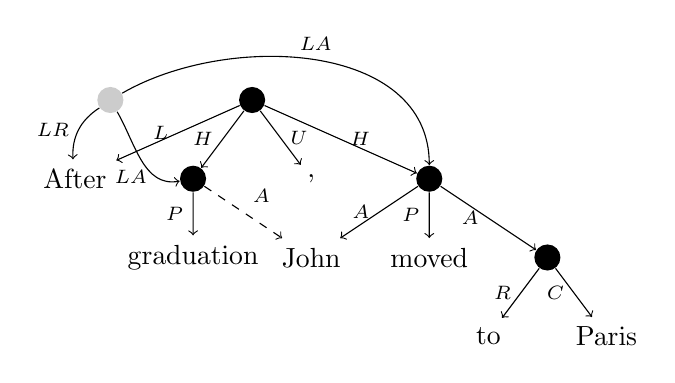
\begin{tikzpicture}[level distance=10mm, ->]
    \node (ROOT) [fill=black, circle] {}
      child {node (After) {After} edge from parent node[left] {\scriptsize $L$}}
      child {node (graduation) [fill=black, circle] {}
      {
        child {node {graduation} edge from parent node[left] {\scriptsize $P$}}
      } edge from parent node[left] {\scriptsize $H$} }
      child {node {,} edge from parent node[right] {\scriptsize $U$}}
      child {node (moved) [fill=black, circle] {}
      {
        child {node (John) {John} edge from parent node[left] {\scriptsize $A$}}
        child {node {moved} edge from parent node[left] {\scriptsize $P$}}
        child {node [fill=black, circle] {}
        {
          child {node {to} edge from parent node[left] {\scriptsize $R$}}
          child {node {Paris} edge from parent node[left] {\scriptsize $C$}}
        } edge from parent node[left] {\scriptsize $A$} }
      } edge from parent node[right] {\scriptsize $H$} }
      ;
    \node (LKG) at (-1.8,0) [fill=black!20, circle] {};
    \draw[dashed,->] (graduation) to node [auto] {\scriptsize $A$} (John);
    \draw[bend right] (LKG) to node [auto, left] {\scriptsize $LR$} (After);
    \draw (LKG) to[out=-60, in=190] node [below] {\scriptsize $LA\quad$} (graduation);
    \draw (LKG) to[out=30, in=90] node [above] {\scriptsize $LA$} (moved);
  \end{tikzpicture}
  }
  \caption{}
  \label{fig:graduation}
  \end{subfigure}
%  \scalebox{.9}{
%  \begin{tikzpicture}[level distance=12mm, ->,
%      every node/.append style={midway}]
%    \node (ROOT) [fill=black, circle] {}
%      child {node (John) {John} edge from parent node[left] {\scriptsize $A$}}
%      child {node {decided} edge from parent node[left] {\scriptsize $P$}}
%      child {node (totakeaquickshower) [fill=black, circle] {}
%      {
%        child {node {to} edge from parent node[left] {\scriptsize $F$}}
%        child {node (takeashower) [fill=black, circle] {}
%        {
%          child {node {take} edge from parent node[left] {\scriptsize $C$}}
%          child {node {a} edge from parent node[right] {\scriptsize $F$}}
%          child {node (quick) {quick} edge from parent[white]}
%          child {node {shower} edge from parent node[right] {\scriptsize $C$}}
%        } edge from parent node[right] {\scriptsize $P$} }
%      } edge from parent node[left] {\scriptsize $A$} }
%      ;
%    \draw[bend left,dashed,->] (takeashower) to node [auto] {\scriptsize $A$} (John);
%    \draw[bend left,->] (totakeaquickshower) to node [auto] {\scriptsize $D$} (quick);
%  \end{tikzpicture}
%  }
  \begin{subfigure}[t]{.5\textwidth}
  \centering
  \scalebox{.9}{
  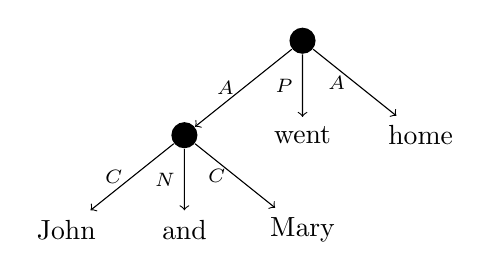
\begin{tikzpicture}[level distance=12mm, ->,
      every node/.append style={midway}]
    \node (ROOT) [fill=black, circle] {}
      child {node [fill=black, circle] {}
      {
        child {node {John} edge from parent node[left] {\scriptsize $C$}}
        child {node {and} edge from parent node[left] {\scriptsize $N$}}
        child {node {Mary} edge from parent node[left] {\scriptsize $C$}}
      } edge from parent node[left] {\scriptsize $A$} }
      child {node {went} edge from parent node[left] {\scriptsize $P$}}
      child {node {home} edge from parent node[left] {\scriptsize $A$}}
      ;
  \end{tikzpicture}
  }
  \caption{}
  \label{fig:home}
  \end{subfigure}
  \begin{subfigure}[t]{.5\textwidth}
  \centering
  \scalebox{.9}{
  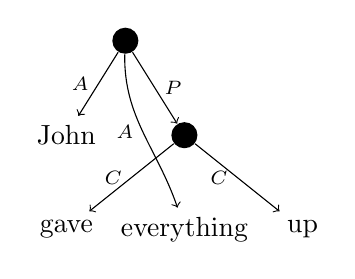
\begin{tikzpicture}[level distance=12mm, ->,
      every node/.append style={midway}]
    \node (ROOT) [fill=black, circle] {}
      child {node {John} edge from parent node[left] {\scriptsize $A$}}
      child {node [fill=black, circle] {}
      {
      	child {node {gave} edge from parent node[left] {\scriptsize $C$}}
      	child {node (everything) {everything} edge from parent[white]}
      	child {node {up} edge from parent node[left] {\scriptsize $C$}}
      } edge from parent node[right] {\scriptsize $P$} }
      ;
    \draw[bend right,->] (ROOT) to[out=-20, in=180] node [left] {\scriptsize $A$} (everything);
  \end{tikzpicture}
  }
  \caption{}
  \label{fig:gave}
  \end{subfigure}
  \label{fig:examples}
  \caption{\small
  UCCA graphs for three example sentences:
  ``After graduation, John moved to Paris'',
  ``John and Mary went home''
  and ``John gave everything up.''
  % and ``John decided to take a quick shower.''
  The first sentence includes a remote edge (dashed),
  resulting in ``John'' having two parents, and
  a linkage relation (gray node and its outgoing edges).
  The second sentence includes a coordination construction (``John and Mary'').
  The third sentence includes a discontinuous unit (``gave ... up'').
  Legend: $P$ -- a Scene's main relation, $A$ -- participant,
  $L$ -- inter-scene linker, $H$ -- linked Scene, $F$ -- function unit,
  $LA$ -- link argument, $LR$ -- link relation.
  Pre-terminal nodes are omitted for brevity.
}
\end{figure}

\com{
\begin{figure*}
\begin{adjustbox}{width=\textwidth}
  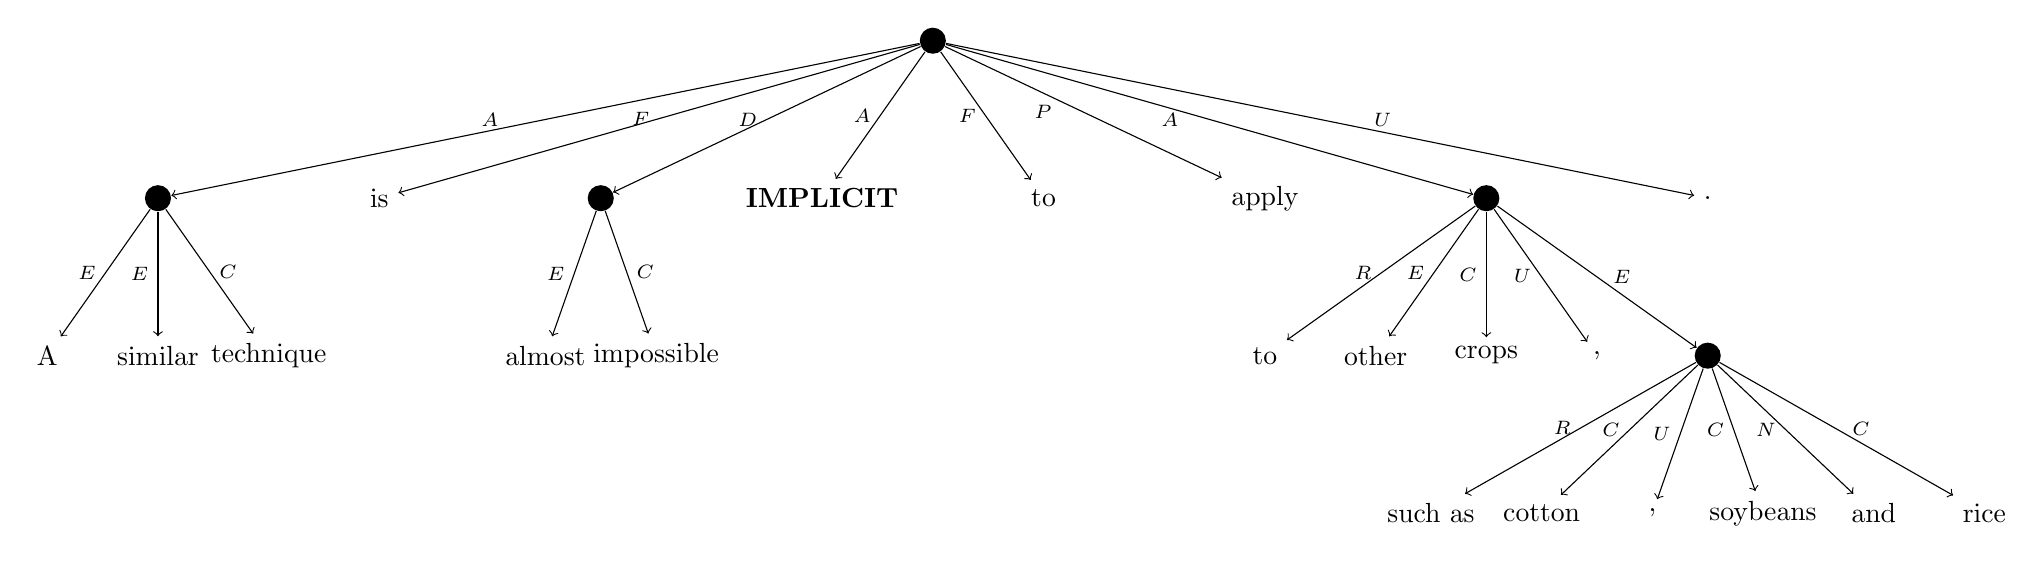
\begin{tikzpicture}[level distance=20mm, ->,
  level 1/.style={sibling distance=8em},
  level 2/.style={sibling distance=4em},
  level 3/.style={sibling distance=4em}]
    \node (ROOT) [fill=black, circle] {}
      child {node [fill=black, circle] {}
      {
        child {node {A} edge from parent node[left] {\scriptsize $E$}}
        child {node {similar} edge from parent node[left] {\scriptsize $E$}}
        child {node {technique} edge from parent node[right] {\scriptsize $C$}}
      } edge from parent node[left] {\scriptsize $A\quad$ \hspace{1mm} } }
      child {node {is} edge from parent node[left] {\scriptsize $F$}}
      child {node [fill=black, circle] {}
      {
        child {node {almost} edge from parent node[left] {\scriptsize $E$}}
        child {node {impossible} edge from parent node[right] {\scriptsize $C$}}
      } edge from parent node[left] {\scriptsize $D$} }
      child {node {\textbf{IMPLICIT}} edge from parent node[left] {\scriptsize $A$}}
      child {node {to} edge from parent node[left] {\scriptsize $F$}}
      child {node {apply} edge from parent node[left] {\scriptsize $P\quad$}}
      child {node [fill=black, circle] {}
      {
        child {node {to} edge from parent node[left] {\scriptsize $R$}}
        child {node {other} edge from parent node[left] {\scriptsize $E$}}
        child {node {crops} edge from parent node[left] {\scriptsize $C$}}
        child {node {,} edge from parent node[left] {\scriptsize $U$}}
        child {node [fill=black, circle] {}
        {
          child {node {such as} edge from parent node[left] {\scriptsize $R$}}
          child {node {cotton} edge from parent node[left] {\scriptsize $C$}}
          child {node {,} edge from parent node[left] {\scriptsize $U$}}
          child {node {soybeans} edge from parent node[left] {\scriptsize $C$}}
          child {node {and} edge from parent node[left] {\scriptsize $N$}}
          child {node {rice} edge from parent node[right] {\scriptsize $\; C$}}
        } edge from parent node[right] {\scriptsize $\; E$ \hspace{1mm} } }
      } edge from parent node[left] {\scriptsize $A\;$ \hspace{1mm} } }
      child {node {.} edge from parent node[right] {\scriptsize $\quad \quad U$}}
      ;
  \end{tikzpicture}
\end{adjustbox}
\caption{\label{fig:ucca_example2}
  UCCA graph for the sentence ``A similar technique is almost impossible to
  apply to other crops, such as cotton, soybeans and rice.''
  The sentence was used by Oepen et al. (2015) to compare between the difference schemes. The sentence includes a single Scene, whose main relation is ``apply'', a secondary relation ``almost impossible'', as well as two complex arguments: ``a similar technique'' and the coordinated argument ``such as cotton, soybeans, and rice.''
}
\end{figure*}
}

\paragraph{Broad-coverage Semantic Representation.}
Earlier work on statistical broad-coverage semantic parsing has mostly
concentrated on shallow semantic analysis, mainly addressing semantic
role labeling of verbal argument structures. 
Recently, work has shifted to parsing of more elaborate representations, that account
for a wider range of phenomena, such as inter-clause relations and non-verbal predicates.
Most work has addressed parsing sentences into Abstract Meaning Representations (AMRs),
which represents sentences as directed graphs, without
grounding their semantic sub-parts in the sentence's words and constituents.
Examples of AMR parsers include 
\cite{flanigan2014discriminative,vanderwende2015amr,pust2015parsing,artzi2015broad}. 

While sharing much of this work's motivation, AMR parsing differs from broad-coverage
semantic constituency parsing in two important ways.
First, AMR uses an open-ended and fine-grained ontology for defining its categories,
rather than a uniform closed inventory.
%It poses difficulties as it conflates
%a wide variety of linguistic phenomena into a single representation.
Second, not grounding the text within the semantic representation, 
requires that the alignment between words and logical symbols be automatically
(and imprecisely) detected, and complicates the parsing task.
Transition-based approach has been applied to AMR parsing by \newcite{wang2015transition},
but their approach involved first syntactically parsing the input, and then converting
the resulting tree into an AMR, unlike the \textsc{bcs} parser which performs parsing in a single step.

Another line of work that addresses parsing into elaborate semantic structures
is that of Broad-coverage Semantic Dependency Parsing (SDP) \cite{oepen2014semeval,oepen2015semeval}.
Like AMR, SDP also addresses a wide range of argument structures (including verbal, nominal and
adjectival ones) and the inter-relations between them, but uses word-to-word dependency structures.
Three representation approaches have been studied:
the Prague Dependency Treebank tectogrammatical layer \cite{bohmova2003prague},
HPSG-derived parsers using the Enju parser\footnote{See \url{http://kmcs.nii.ac.jp/enju/}.},
and dependencies derived from the Lingo ERG Minimal Recursion Semantics representations \cite{Flic:02}.
%An alternative line of work tackles parsing into grounded semantic representations.
%Most work of this strand represent semantics using dependency structures,
%as has been explored in two recent SemEval shared tasks \cite{oepen2014semeval,oepen2015semeval}.
Bi-lexical dependencies are appealing for semantic representation, partly due to
their structural simplicity and the strong parsing methods they allow for.
However, their assumption that each semantic unit has a unique head is
problematic for representing several frequent constructions which have no clear
head, such as coordination, prepositional phrases and multi-word expressions,
leading to unsystematic treatment of these cases \cite{schwartz2011neutralizing,Ivanova2012who,tsarfaty2012cross}.
% , which results in conceptual and practical problems 

(for discussion of this point in the context of syntactic parsing, see
\cite{kallmeyer2013data,pitler2015linear})

\paragraph{Universal Conceptual Cognitive Annotation.}\label{subsec:ucca}
Taking a constituency-based approach to semantic parsing,
we use the annotated UCCA corpora, a broad-coverage semantic annotation scheme that
represents predicate-argument structures (verbal, nominal, adjectival and others),
the inter-relations between them, in addition to other major semantic phenomena.
UCCA builds on an established framework
for typological description, ``Basic Linguistic Theory''
\cite{Dixon:10b,Dixon:10a,Dixon:12}, as well as on the Cognitive Linguistics literature,
and defines a set of coarse-grained, cross-linguistically applicable distinctions.
UCCA has demonstrated applicability to multiple languages, including English, French, German and
Czech, support for rapid annotation, and semantic stability in translation: UCCA
annotations of translated text usually contain the same set of relationships
\cite{sulem2015conceptual}.

Formally, a UCCA structure is a constituency DAG, whose leaves correspond to the words of the text. The
nodes of the graph, called ``units'', are either terminals or several elements (not necessarily contiguous)
jointly viewed as a single entity according to some semantic or cognitive consideration.
Edges bear a category, indicating the role of the sub-unit in the relation that the parent represents. 
The most basic notion is the {\it Scene}, which describes a movement, an action or a state.
Each Scene contains one main relation, or anchor, as well as one or more participants.
For example, the sentence ``After graduation, John moved to Paris'' contains two Scenes,
whose main relations are ``graduation'' and ``moved''. The participant ``John'' is a part of both Scenes, while ``Paris'' only of the latter.
The two Scenes in this sentence are both arguments in the \textit{linkage relation} ``After'', in this case expressing temporal linkage between them.
For example, the sentence ``John decided to take a shower'' contains two Scenes, whose main relations are ``decided'' and ``take a shower'', and where the second Scene is a participant in the first.
The participant ``John'' is a part of both Scenes, but is marked as a \textit{remote} participant in
the second, since it is not explicit in the second clause.
Further categories account for relations between Scenes and
the internal structures of complex arguments (e.g., coordination) and relations (e.g., complex adverbials, such a ``very clearly'').
UCCA graphs for both examples are given in \figref{fig:ucca_example1}\footnote{
UCCA graphs may contain implicit units that have no correspondent in the text.
Such units serve in UCCA to represent implicit relations and participants,
such as the agent in passive sentences.
We defer the parsing of these units to future work,
as it is likely to require different machinery than
those explored here \cite{roth2015inducing}.}.
  
%Another example for a UCCA-annotated sentence is shown in \figref{fig:ucca_example2}.

\paragraph{Related Semantic and Syntactic Parsing Work.}
Semantic parsing methods can be largely partitioned into grammar-based and grammarless methods.
Within the grammar-based literature, most work relied on Combinatory Categorial Grammar (CCG)
\cite{Steedman:00}, which allows to compute semantic structure compositionally from the
syntactic derivations. Notable examples include the Boxer parser \cite{bos2005towards}
and the AMR parser by \newcite{artzi2015broad}.
Other examples include parsing with Hyperedge Replacement Grammars
\cite{jones2012semantics,chiang2013parsing,peng2015synchronous} and
graph grammars \cite{koller2015semantic}.
A different line of work takes a discriminative, grammarless approach,
pursuing either graph-based methods that predict the highest ranking graph
(tree or DAG) that satisfies a given set of constraints
(e.g., \newcite{flanigan2014discriminative} for AMR parsing)
or a transition-based method that builds the parse incrementally following a series of local
decisions \cite[and much subsequent work]{Nivre03anefficient}.

Despite being based on local decisions, transition-based methods have yielded excellent
results in a variety of parsing tasks. Within syntactic dependencies parsing, transition-based methods
have been successfully applied to corpora in many languages and domains, yielding some
of the best reported results \cite{dyer2015transition,ballesteros2015improved}. 
The approach has also yielded results comparable with the state-of-the-art when applied
to constituency parsing \cite{sagae2005classifier,zhu2013fast}, and has been recently extended to
discontinuous constituency parsing \cite{maier2015discontinuous},
yielding improvements over in the parsing of discontinuous constituents in German.
Transition-based parsers have also been developed for dependency DAG structures
\cite{sagae2008shift,tokgoz2015transition} and CCG parsing \cite{ambati2015incremental}.
Nevertheless, there are no constituency DAG parsers, a gap this work addresses.

%\oa{Who to compare to? (we take a transition-based approach; later we discuss,
%  without comparing, to grammar-based
%  or graph-based approaches)
%  Constituency parsers that meet some of the criteria: Wolfgang's (all but multiple parents),
%        which is state-of-the-art on Negra discontiguous units.
%        There are no multiple parent constituency parsers! (so we can't compare)
%%  Dependency parsers: there are the standard ones (done!), there is MALT non-projective, and there is not MALT with multiple parents. There are other dependency with multiple parents: tokgoez and erdigit (based on earlier work by sagae and tsujii) -- we're trying to get their code.
%  
%  We'll also say that future work will address other languages, ...
%  Evaluation specifically on multiple parents, and on discontiguous.
%  Future work: LSTM-version of our parser, conversion from t-layer parsers and such.
%}

% ADL comment: I removed these paragraphs because I think the text should zero in on precisely what our research methods, without dwelling on background/ previous work, esp. this early in the text. If this appears at all it should be briefly summarized at the end; say how it informs UCCA, but don't dwell on it.

%Ascribing structure to text or speech is an essential component in any linguistic analysis and computational modeling of language. Large-scale structurally annotated corpora began to emerge in the early 90s, and have made an enormous impact on computational linguistics. 
%Most structurally annotated corpora hitherto focused on formulating a set of distinctions applicable to a certain language or genre. A partial reason for the language specificity of the schemes is that most existing treebanks tend to reflect first and foremost syntactic structures, which vary dramatically between languages. 

%This difficulty has resulted in recent years in two major types of work. 
%One is cross-linguistically applicable {\bf syntactic} representation, much of which is currently addressed under the Universal Dependencies project\footnote{\url{http://universaldependencies.github.io/docs/}}. 
%The other is cross-linguistically applicable {\bf semantic} schemes, expressing a shared level of semantic representation, which are therefore more in line with the purposes of this proposal. The most widely used of these is FrameNet \cite{Fillmore:71}, which focuses on lexical semantics with emphasis on cross-linguistic validity \cite{boas2009multilingual}.
%(though see \cite{goddard2011semantic} for critique). 
%While proving a valuable resource, it has limited coverage, even for English, the most studied language \cite{palmer2010evaluating}, and focuses almost exclusively on argument structure phenomena.

%The Abstract Meaning Representation (AMR) project \cite{AMR:13}, which has attracted considerable attention recently, also provides semantic annotation in the form of elaborate graphs, representing distinctions of various types (including word sense disambiguation, argument structure, compositionality, co-reference). AMR is not optimal for our purposes as it conflates a wide variety of linguistic phenomena into a single unlayered representation, and reflects highly fine-grained phenomena, resulting in many cross-linguistic divergences \cite{XUE14not}.
%AMR poses further difficulties in not embedding the text within the semantic representation, often requires that this correspondence will be automatically (and hence imprecisely) derived.
%(e.g., \cite{flanigan2014discriminative}).

%\subsubsection{Universal Cognitive Conceptual Annotation}

%The inadequacy of string-to-string methods in SMT has resulted in structure aware methods that construe translation as the learning of a function between texts augmented with structural annotation, generally relfecting their syntactic or other structural propoerties. In this sense, imposing linguistic structure on the source and target texts is useful if the translation function between these structures is sufficiently constrained to allow its statistical learning. Semantic representation is an appealing source of cross-linguistically applicable structures, since a major goal of translation is preserving the meaning of the source text.

%UCCA shares AMR's [isn't AMR English-centric?] goal of a cross-linguistically applicable scheme that can benefit semantics-based MT, but is better suited for our purposes in two respects. First, UCCA builds on typological theory and provides empirical support for its cross-linguistic applicability through its application to a sizable corpora in English and French, using the same set of categories \cite{sulem2015conceptual}, in addition to further preliminary experiments in German, Hebrew and Czech. Second, it is built in {\it layers}, each addressing a specific module of semantic distinctions, such as argument-structural, information-theoretic or logical distinctions, which allows more controlled experiments, important in these early stages of semantics-based MT.



%Syntactic dependency trees can in general be non-projective. Graph-based parsers are able to produce such trees, but many transition-based parsers assume projectivity to improve the performance and efficiency of the parser: the number of transitions in such parsers is always $2n$ where $n$ is the number of tokens \cite{nivre2004incrementality}. However, non-projective dependency trees can also be parsed by transition-based parsers in empirical linear time \cite{nivre2009non}.

%In a UCCA graph, labels appear on the edges, whereas nodes are unlabeled. If all the nodes are known, parsing is the same as inducing a graph on them with the correct edge labels. In dependency parsing, a graph is induced on the set of nodes consisting of the tokens in the sentence (and the \textsc{ROOT} symbol). Therefore, it seems that techniques from dependency parsing can be used for UCCA parsing as well.

%\paragraph{Other Semantic Schemes.}

%Although the labels in a UCCA graph are on the edges, it is similar to phrase structure grammar: non-terminal units are internal nodes in the graph, rather than all the edges being between words in the original sentence. In a constituency tree, constituents form a hierarchy above the words of the sentence.

%Methods for constituent parsing can also be useful for UCCA parsing, but the common chart-based approach is also $\mathcal{O}(n^3)$ at best. However, there are also transition-based constituent parsers~\cite{zhu2013fast} with linear run-time complexity.

%Like standard dependency parsers, transition-based constituent parsers are generally unable to produce \textit{discontinuous constituents} (the equivalent of non-projective dependency trees). However, Maier~\shortcite{maier2015discontinuous} introduced a transition-based constituent parsing with a \textsc{swap} transition to allow discontinuous parsing.\footnote{https://github.com/wmaier/uparse}




%%%%%%%%%%%%%%%%%%%%%%%%%%%%%%%%%%%%%%%%%%%%%%%%%%%%%%%%%%%%%%%
\section{Conversion-Based Parsing}\label{sec:conversion_approach}

We begin by assessing the ability of existing technology to address the task,
by taking a conversion-based approach. Training proceeds by 
converting the constituency DAGs into the target representation,
and training an existing parser for that representation on the converted representations.
We test the parsers by applying the resulting parser to the text of the test set,
and converting back to the original constituency DAG format, where they are compared
with the gold standard.
The amount of information lost by this back and forth conversion is discussed in
\secref{sec:experiments}.

\paragraph{Notation.}
Let $L$ be the set possible edge labels.
A constituency DAG is a directed acyclic graph $G=(V,E, \ell)$
over a sequence of tokens $w_1, \ldots, w_n$,
where $\ell:E\to L$ is a function of \textit{edge labels}.
For each token $w_i$ ($i=1, \ldots, n$) there exists a leaf (or a terminal) $t_i \in V$.

\paragraph{Conversion to Constituency Trees.}
We convert constituency DAGs to constituency trees by removing a subset of the edges.
As the original constituency DAGs may contain discontinuous units, the resulting trees
may also have contain such units.
Specifically, when converting UCCA structures, we note that UCCA marks one of the incoming edges
for each non-root as ``primary'' and the others as ``remote'' and ``linkage'' edges.
We thus remove all remote and linkage edges, in addition to nodes that are disconnected
from the graph as a result of this removal. 
The inverse conversion from trees to graphs is simply the identity function.

\paragraph{Conversion to Dependency Trees.}\label{subsec:con2dep}
In the conversion to dependency trees, we first convert semantic constituency graphs
to constituency trees using the above procedure, and then convert the result to dependency trees. 
Assume $T_c=(V_c,E_c,\ell_c)$ is a constituency tree with labels $\ell_c:E_c~\rightarrow~L$,
where $L$ is the set of possible labels.
The conversion from $T$ to a dependency tree involves the removal of
all non-terminals from $T$ and the addition of edges between terminals.
The nodes of the converted dependency tree are simply the terminals of $T$.

We define a linear order over possible edge labels $L$.
For each node $u \in V$, denote with $h(u)$ its child with the highest edge label.
Denote with $h^*(u)$ the terminal reached by recursively applying of $h(\cdot)$ over $u$.
For each terminal $t$, we define $n(t)$ as the highest
non-terminal such that $t=h^*(n(t))$, i.e.,
$n(t)$ is the only node such that $t=h^*(n(t))$ and $t \neq h^*(\mathrm{Parent}_c(n(t)))$.
The head of $t$ according to the dependency graph is
the terminal $h^*(\mathrm{Parent}_c(n(t)))$.
The complete algorithm is given in Algorithm~\ref{alg:con2dep}.

We note that this conversion procedure is simpler than the
head percolation procedure used for converting syntactic constituency
trees to dependency trees.
This is because $h(u)$ of a node $u$ (similar to $u$'s head-containing child),
depends only on the label of the edge $(h(u),u)$, and not on the sub-tree spanned by $u$,
because edge labels in UCCA directly express the role of the child in the parent unit, and
are thus sufficient for determining which of $u$'s children contains the head node.
%This is appropriate, since edges in a semantic constituency graph express the relation between units,
%whereas in syntactic constituency trees the identity of a node depends on the nodes below it.


\begin{algorithm}[t]
 \KwData{constituency tree ${T_c}=(V_c,E_c,\ell_c)$}
 \KwResult{dependency tree $T_d=(V_d,E_d,\ell_d)$}
 \ForEach{$u \in V_c$} {
  $h(u) \leftarrow \argmin_v \mathrm{Priority}(\ell_c(u,v))$\;
 }
 $V_d \leftarrow \mathrm{Terminals}({T_c})$,
 $E_d \leftarrow \emptyset$\;
 \ForEach{$t \in V_d$} {
  $u \leftarrow t$\;
  \While{$u=h(\mathrm{Parent}_c(u))$} {
  	$h^*(u) \leftarrow t$\;
  	$u \leftarrow \mathrm{Parent}_c(u)$\;
  }
  $n(t) \leftarrow h(u)$\;
 }
 \ForEach{$t \in V_d$} {
  $u \leftarrow \mathrm{Parent}_c(n(t))$\;
  $t^\prime \leftarrow h^*(u)$\;
  $E_d \leftarrow E_d \cup \{(t^\prime, t)\}$\;
  $\ell_d (t^\prime, t) \leftarrow \ell_c(u, n(t))\}$\;
 }
 \caption{Constituency to dependency conversion procedure.}
 \label{alg:con2dep}
\end{algorithm}

The inverse conversion introduces non-terminal nodes back into the tree.
As the distinction between low- and high-attaching nodes is lost in the constituency to
dependency conversion, we heuristically assume that attachments are always
high-attaching.

Assume $T_d=(V_d,E_d,\ell_d)$ is a dependency tree.
We begin by creating a root node $r$.
Then, iterating over $V_d$ in topological order,
we add its members as terminals to the constituency tree
and create a pre-terminal parent for each,
with an edge labeled as \textit{Terminal} between them.
The parents of the pre-terminals are determined by the terminal's parent in the dependency
tree: if a dependency node $t$ is a child of the root in $T_d$, then $t$'s pre-terminal will also be a child of the root node. Otherwise, $t$'s pre-terminal is the child of the pre-terminal associated with $t$'s head in $T_d$. We add an intermediate node in between if $t$ has any dependents in $T_d$,
to allow adding their pre-terminals as children.
Edge labels for the intermediate edges are determined by a rule-based function, denoted by $\mathrm{Label}(u)$.
In practice, it mostly selects the label $C$ (Center).

\begin{algorithm}
 \KwData{dependency tree $T_d=(V_d,E_d,\ell_d)$}
 \KwResult{constituency tree $T_c=(V_c,E_c,\ell_c)$}
 $r \leftarrow \mathrm{Node()}$\;
 $V_c \leftarrow \{r\}$,
 $E_c \leftarrow \emptyset$\;
 \ForEach{$t \in \mathrm{TopologicalSort}(V_d)$} {
  $u \leftarrow \mathrm{Node()}$\;
  $V_c \leftarrow V_c \cup \{u, t\}$\;
  $E_c \leftarrow E_c \cup \{(u, t)\}$\;
  $\ell_c(u,t)\leftarrow\mathit{Terminal}$\;
  $t^\prime \leftarrow \mathrm{Parent}_d(t)$\;
  \eIf{$t^\prime = \textsc{Root}$} {
   $E_c \leftarrow E_c \cup \{(r, u)\}$\;
   $\ell_c(r, u) \leftarrow \mathrm{Label}(r,u)$\;
  } {
   \eIf{$\exists v \in V_d : (t,v) \in E_d$} {
    $u^\prime \leftarrow \mathrm{Node()}$\;
    $E_c \leftarrow E_c \cup \{(u^\prime, u)\}$\;
    $\ell_c(u^\prime, u) \leftarrow \mathrm{Label}(u^\prime, u)$\;
   } {
    $u' \leftarrow u$\;
   }
   $p \leftarrow \mathrm{Parent}_c(t^\prime)$\;
   $E_c \leftarrow E_c \cup \{(p, u^\prime)\}$\;
   $\ell_c(p, u^\prime) \leftarrow \ell_d(t^\prime, t)$\;
  }
 }
 \caption{Dependency to constituency conversion procedure.}
 \label{alg:dep2con}
\end{algorithm}


%%%%%%%%%%%%%%%%%%%%%%%%%%%%%%%%%%%%%%%%%%%%%%%%%%%%%%%%%%%%%%%
\section{Constituency DAG Parsing}\label{sec:direct_approach}

We now turn to the direct approach for parsing semantic constituency graphs. Given a sequence
of tokens $w_1, \ldots, w_n$, we directly predict a DAG $G$ whose leaves
correspond to  $w_1, \ldots, w_n$.

%We define a transition system for constituency DAG parsing as a quadruple $S=(C,T,c_s,C_t)$, where
%\begin{enumerate}
% \item $C$ is a set of \textit{configurations}.
% \item $T$ is a set of \textit{transitions}.
% \item $c_s$ is a function mapping a sequence of tokens to an \textit{initial state} in $C$.
% \item $C_t$ is a set of \textit{terminal configurations}.
%\end{enumerate}

In transition-based (also called \textit{shift-reduce}) parsing, the input is scanned from left to right.
The output is created incrementally by applying a \textit{transition} at each step to the parser state,
defined using three data structures: a buffer $B$ of tokens and nodes to be processed,
a stack $S$ of nodes currently being processed,
and a graph $G=(V,E,\ell)$ of constructed nodes and labeled edges.
In addition, some states are marked as \textit{terminal}, meaning that $G$ is the final output.
A classifier is used at each step to select the next transition based on features
which encode the parser's current state.

\paragraph{Transition Set.}
Parsing starts with a single node in the stack (the root node), and the input tokens
$w_1, \ldots, w_n$ in the buffer. The set of transitions is given in \figref{fig:transitions}.

\begin{figure*}
\begin{adjustbox}{width=\textwidth,margin=3pt,frame}
\begin{tabular}{llll|l|llllc|c}
\multicolumn{5}{c|}{\textbf{\small Initial State}} & \multicolumn{6}{c}{\textbf{\small Final State}} \\
\textbf{\footnotesize Stack} & \textbf{\footnotesize Buffer} & \textbf{\footnotesize Nodes} & \multicolumn{1}{l}{\textbf{\footnotesize Edges}} & \multicolumn{1}{c|}{\textbf{\footnotesize Terminal?}} & \textbf{\footnotesize Stack} & \textbf{\footnotesize Buffer} & \textbf{\footnotesize Nodes} & \textbf{\footnotesize Edges} & \multicolumn{1}{c}{\textbf{\footnotesize Terminal?}} \\
$[\mathrm{root}]$ & $w_{1:n}$ & \multirow{2}{40pt}{$\{\mathrm{root}\} \cup w_{1:n}$} & \multicolumn{1}{l}{$\emptyset$} & \multicolumn{1}{c|}{$-$} & $\emptyset$ & $\emptyset$ & $V$ & $E$ & \multicolumn{1}{c}{$+$} \\ 
\multicolumn{5}{c|}{} \\
\multicolumn{5}{c|}{} \\
\hline
%\end{tabular}
%\end{adjustbox}
%\begin{adjustbox}{width=\textwidth,frame}
%\begin{tabular}{llll|l|llllc|l}
\multicolumn{4}{c|}{\textbf{\small Before Transition}} & \textbf{\small Transition} & \multicolumn{5}{c|}{\textbf{\small After Transition}} & \textbf{\small Condition} \\
\textbf{\footnotesize Stack} & \textbf{\footnotesize Buffer} & \textbf{\footnotesize Nodes} & \textbf{\footnotesize Edges} & & \textbf{\footnotesize Stack} & \textbf{\footnotesize Buffer} & \textbf{\footnotesize Nodes} & \textbf{\footnotesize Edges} & \textbf{\footnotesize Terminal?} & \\
$S$ & $x \;|\; B$ & $V$ & $E$ & \textsc{Shift} & $S \;|\; x$ & $B$ & $V$ & $E$ & $-$ & \\
$S \;|\; x$ & $B$ & $V$ & $E$ & \textsc{Reduce} & $S$ & $B$ & $V$ & $E$ & $-$ & \\
$S \;|\; x$ & $B$ & $V$ & $E$ & \textsc{Node$_X$} & $S \;|\; x$ & $y \;|\; B$ & $V \cup \{ y \}$ & $E \cup \{ (y,x)_X \}$ & $-$ &
$x \neq \mathrm{root}$ \\
%$S \;|\; x$ & $B$ & $V$ & $E$ & \textsc{Implicit$_X$} & $S \;|\; x$ & $y^* \;|\; B$ & $V \cup \{ y^* \}$ & $E \cup \{ (x,y^*)_X \}$ & $-$ &
%$x \not\in w_{1:n}$ \\
$S \;|\; y,x$ & $B$ & $V$ & $E$ & \textsc{Left-Edge$_X$} & $S \;|\; y,x$ & $B$ & $V$ & $E \cup \{ (x,y)_X \}$ & $-$ &
\multirow{4}{50pt}{\vspace{-5mm}\[\left\{\begin{array}{l}
x \not\in w_{1:n},\\
y \neq \mathrm{root},\\
x \not\leadsto_G y
\end{array}\right.\]} \\
$S \;|\; x,y$ & $B$ & $V$ & $E$ & \textsc{Right-Edge$_X$} & $S \;|\; x,y$ & $B$ & $V$ & $E \cup \{ (x,y)_X \}$ & $-$ & \\
$S \;|\; y,x$ & $B$ & $V$ & $E$ & \textsc{Left-Remote$_X$} & $S \;|\; y,x$ & $B$ & $V$ & $E \cup \{ (x,y)_X^* \}$ & $-$ & \\
$S \;|\; x,y$ & $B$ & $V$ & $E$ & \textsc{Right-Remote$_X$} & $S \;|\; x,y$ & $B$ & $V$ & $E \cup \{ (x,y)_X^* \}$ & $-$ & \\
$S \;|\; x,y$ & $B$ & $V$ & $E$ & \textsc{Swap} & $S \;|\; y$ & $x \;|\; B$ & $V$ & $E$ & $-$ &
$\mathrm{i}(x) < \mathrm{i}(y)$ \\
$[r]$ & $\emptyset$ & $V$ & $E$ & \textsc{Finish} & $\emptyset$ & $\emptyset$ & $V$ & $E$ & $+$ & \\
\end{tabular}
\end{adjustbox}
\caption{\label{fig:transitions}
  The transition set of the \textsc{bcs} parser. Following standard practice,
  we write the stack with its top to the right and the buffer with its head to the left.
  $(\cdot,\cdot)_X$ denotes an $X$-labeled edge, $(\cdot,\cdot)_X^*$ a remote $X$-labeled edge,
  and $x^*$ an implicit node. $\mathrm{i}(x)$ is a running index for the created nodes.
}
\end{figure*}

In addition to the standard \textsc{Shift} and \textsc{Reduce} operations, 
we follow previous work in transition-based constituency parsing \cite{zhu2013fast}, and include the \textsc{Node} transition for creating new non-terminal nodes.
Concretely, \textsc{Node$_X$} creates a new node on the buffer as a parent of the first element on the stack, with an $X$-labeled edge.
%\textsc{Implicit$_X$} acts similarly, but the created node is a child instead,
%and is marked as \textit{implicit}, representing a unit that does not appear explicitly in the text.

\textsc{Left-Edge$_X$} and \textsc{Right-Edge$_X$} create a primary new $X$-labeled edge between the first two elements on the stack, where the parent is the left or the right node, respectively. As a UCCA node may only
have one incoming primary edge, \textsc{Edge} transitions are disallowed where the child node already
has an incoming primary edge.
\textsc{Left-Remote$_X$} and \textsc{Right-Remote$_X$} do the same, but the created edge is marked as \textit{remote}. We distinguish between these two pairs of transitions, for the parser to be able to predict whether an edge is a primary or a remote one.
In order to allow nodes to have multiple parents, node and edge transitions do not automatically
apply \textsc{Reduce}. This is in line with other work on
transition-based DAG dependency parsing \cite{sagae2008shift,tokgoz2015transition}.
Once all edges for a particular node have been created, it is removed from the stack
by applying \textsc{Reduce}.

\textsc{Swap} allows handling discontinuous nodes, by popping the second
node on the stack and adding it to the top of the buffer, as with the similarly
named transition in previous work \cite{nivre2009non,maier2015discontinuous}.
Finally, \textsc{Finish} pops the root node and marks the state as terminal.

\paragraph{Features.}
\label{subsec:features}

\figref{fig:features} presents the feature templates used by the parser.
For some of the features, we used the notion of \textit{head word},
defined by the $h^*(\cdot)$ function (\secref{subsec:con2dep}).
While head words are not explicitly represented in the UCCA scheme, these
features proved useful as means of encoding bi-lexical dependencies.

In addition to the binary features defined by the feature templates,
we employ a real-valued feature corresponding to the ratio between the number of terminals to number of nodes
in the graph $G$. This novel feature serves as a regularizer for the creation of new nodes, and should be beneficial for other transition-based constituency parsers too.
Features are generally adapted from the related parsers of \newcite{zhang2009transition,zhu2013fast,tokgoz2015transition} and
\newcite{maier2015discontinuous}, with a small additional set of features encoding relevant information
for the novel \textsc{Left-Remote$_X$} and \textsc{Right-Remote$_X$} transitions.

% and \textsc{Implicit$_X$}

%$s_i$ and $b_i$ stand for the $i$th stack and buffer items respectively, $w$ stands for the head word, $t$ for its POS tag, $e$ for the head incoming edge label. Note that $e$ replaces $c$ (consituent label) from Maier~\shortcite{maier2015discontinuous}, since in UCCA the labels are on the edges rather than the units; and a unit may have more than one incoming edge. $l$ and $r$ ($ll$ and $rr$) represent the leftmost and rightmost children (grand-children) of the element; $u$ handles the unary case.
%Concerning the separator features, $p$ is a unique separator feature between the head words of $s_0$ and $s_1$; $q$ is the count of any separator features between them.
%$x$ denotes the gap type of a subgraph. There are three possible values, either "none" (fully continuous), "pass" (there is a gap at the root, i.e., this gap must be filled later further up in the graph), or "gap" (the root of this graph fills a gap, i.e., its children have gaps, but the root does not). Finally, $y$ is the sum of all gap lengths.

% FEATURES
\begin{figure}
  \begin{adjustbox}{margin=3pt,frame}

\begin{tabular}{>{\small}l}
{Features from \cite{zhang2009transition}:} \\
\textbf{unigrams} \\
$s_0te, s_0we, s_1te, s_1we, s_2te, s_2we, s_3te, s_3we,$ \\
$b_0wt, b_1wt, b_2wt, b_3wt,$ \\
$s_0lwe, s_0rwe, s_0uwe, s_1lwe, s_1rwe, s_1uwe$ \\
\textbf{bigrams} \\
$s_0ws_1w, s_0ws_1e, s_0es_1w, s_0es_1e, s_0wb_0w, s_0wb_0t,$ \\
$s_0eb_0w, s_0eb_0t, s_1wb_0w, s_1wb_0t, s_1eb_0w, s_1eb_0t,$ \\
$b_0wb_1w, b_0wb_1t, b_0tb_1w, b_0tb_1t$ \\
\textbf{trigrams} \\
$s_0es_1es_2w, s_0es_1es_2e, s_0es_1eb_0w, s_0es_1eb_0t,$ \\
$s_0es_1wb_0w, s_0es_1wb_0t, s_0ws_1es_2e, s_0ws_1eb_0t$ \\
\textbf{separator} \\
$s_0wp, s_0wep, s_0wq, s_0wcq, s_0es_1ep, s_0es_1eq,$ \\
$s_1wp, s_1wep, s_1wq, s_1weq$ \\
\\
\textbf{extended} \cite{zhu2013fast} \\
$s_0llwe, s_0lrwe, s_0luwe, s_0rlwe, s_0rrwe,$ \\
$s_0ruwe, s_0ulwe, s_0urwe, s_0uuwe, s_1llwe,$ \\
$s_1lrwe, s_1luwe, s_1rlwe, s_1rrwe, s_1ruwe$ \\
\\
{\footnotesize Features from \cite{maier2015discontinuous}:} \\
\textbf{discontinuous unigrams} \\
$s_0xwe, s_1xwe, s_2xwe, s_3xwe,$ \\
$s_0xte, s_1xte, s_2xte, s_3xte,$ \\
$s_0xy, s_1xy, s_2xy, s_3xy$ \\
\textbf{discontinuous bigrams} \\
$s_0xs_1e, s_0xs_1w, s_0xs_1x, s_0ws_1x, s_0es_1x,$ \\
$s_0xs_2e, s_0xs_2w, s_0xs_2x, s_0ws_2x, s_0es_2x,$ \\
$s_0ys_1y, s_0ys_2y, s_0xb_0t, s_0xb_0w$ \\
\\
{\footnotesize Features from \cite{tokgoz2015transition}:} \\
\textbf{counts} \\
$s_0P, s_0C, s_0wP, s_0wC, b_0P, b_0C, b_0wP, b_0wC$ \\
\textbf{edges} \\
$s_0s_1, s_1s_0, s_0b_0, b_0s_0, s_0b_0e, b_0s_0e$ \\
\textbf{history} \\
$a_0we, a_1we$ \\
\\
\textbf{remote} (Novel, UCCA-specific features) \\
$s_0R, s_0wR, b_0R, b_0wR$
\end{tabular}
\end{adjustbox}

\caption{\small\label{fig:features}
  Feature templates for the \textsc{bcs} parser. Notation:
  $s_i$, $b_i$ are the $i$th stack and buffer items, respectively.
  $w$ and $t$ are the word form and part-of-speech tag of the terminal returned by the $h^*(\cdot)$ function (\secref{subsec:con2dep}).
  $\emph{}$ is the edge label to the node returned by the $h(\cdot)$ function.
  $l$, $r$ ($ll$, $rr$) are the leftmost and rightmost (grand)children, respectively.
  $u$ ($uu$) is the unary (grand)child, when only one exists.
  $p$ is a unique separator punctuation and $q$ is the separator count between $s_0$ and $s_1$.
  $x$ is the gap type (``none'', ``pass'' or ``gap'') at the sub-graph under the current node, and $y$ is the sum of gap lengths \protect\cite{maier2009characterizing}.
  $P$ and $C$ are the number of parents and children, respectively, and $R$ is the number of remote children.
  $a_i$ is the transition taken $i$ steps back.
  All feature templates correspond to binary features.
}
\end{figure}

\paragraph{Training.}
Following \newcite{maier2015discontinuous}, we use a linear classifier, using
the averaged structured perceptron algorithm for training it
\cite{Coll:04} with the \textsc{MinUpdate} \cite{cai2011language} procedure
(i.e., a minimum number of updates to a feature has to occur in training for it
to be included in the model). Inference is performed greedily (i.e., without beam search).

For training the local classifier, we use a dynamic oracle \cite{goldberg2012dynamic},
i.e., an oracle that outputs a set of optimal transitions: when any of them
is applied to the current parser state, the gold
standard graph is reachable from the resulting state.
For example, the oracle would predict a \textsc{Node} transition if the stack 
has on its top a parent in the gold graph that hasn't been created,
but would predict a \textsc{Right-Edge} transition if the second stack
element is a parent of the
first element according to the gold graph and the edge between them hasn't been created.
The transition predicted by the classifier prediction is deemed correct
and is applied to the parser state to reach the subsequent state
if the transition is included in the set of optimal transitions.
Otherwise, a random optimal transition is applied
and the classifier's weights are updated, according to the structured perceptron
update rule.



%%%%%%%%%%%%%%%%%%%%%%%%%%%%%%%%%%%%%%%%%%%%%%%%%%%%%%%%%%%%%%%
\section{Experiments}\label{sec:experiments}

%%%%%%%%%%%%%%%%%%%%%%%%%%%%%%%%%%%%%%%%%%%%%%%%%%%%%%%%%%%%%%%
\subsection{Experimental Setup}

\paragraph{Data.}\label{sec:data}
We conduct our main experiments on the UCCA Wikipedia corpus (henceforth, \textit{Wiki}),
and use the English part of the UCCA \textit{Twenty Thousand Leagues Under the Sea} English-French parallel corpus (henceforth, \textit{20K Leagues}) as
out-of-domain data.\footnote{Both are available at \url{http://www.cs.huji.ac.il/~oabend/ucca.html}}
\tabref{table:data} presents some statistics for the two corpora, demonstrating that while
the \textit{Wiki} corpus is over ten times larger, the overall statistics are
similar.

\begin{table}
  \scalebox{.8}{
\begin{tabular}{l|ccc|c}
& \multicolumn{3}{c}{Wiki} & 20K \\
& \small Train & \small Dev & \small Test & Leagues \\
\hline
\# passages & 281 & 35 & 43 & 154 \\
\# sentences & 4021 & 537 & 608 & 522 \\
\hline
\# nodes & 277,587 & 40,700 & 45,047 & 29,965 \\
\% terminal & 42.41 & 42.8 & 42.66 & 41.23 \\
\% non-term. & 57.59 & 57.20 & 57.34 & 58.77 \\
\% implicit & 0.29 & 0.35 & 0.27 & 0.8 \\
\% linkage & 0.92 & 0.96 & 0.9 & 1.25 \\
\% discont. & 0.52 & 0.55 & 0.47 & 0.79 \\
\% \textgreater 1 parent & 2.29 & 1.89 & 2.21 & 1.98 \\
\hline
\# edges & 272,018 & 39,660 & 44,139 & 28,723 \\
\% primary & 95.37 & 95.70 & 95.90 & 94.48 \\
\% remote & 1.69 & 1.24 & 1.32 & 2.19 \\
\% linkage & 2.94 & 3.06 & 2.78 & 3.33 \\
\hline
\multicolumn{3}{l}{\footnotesize Average per non-linkage non-terminal node} \\
%\# parents & 0.98 & 0.97 & 0.98 & 0.95 \\
\# children & 1.67 & 1.67 & 1.67 & 1.61 
\end{tabular}
}
\caption{\small Statistics of the \textit{Wiki} and \textit{20K Leagues} UCCA corpora.
All counts exclude the root node.
}
\label{table:data}
\end{table}

We use passages of indices up to 655
of the \textit{Wiki} corpus as our training set, passages 656--700 as development set,
and passages 701--695 as in-domain test set.
While UCCA edges can cross sentence boundaries, we adhere to the common
practice in semantic parsing and train our parsers on individual sentences,
discarding inter-relations between them (0.18\% of the edges).
We also discard linkage nodes and edges, as they often express inter-sentence
relations and are thus mostly redundant when applied at the sentence level.
In the out-of-domain experiments, we apply the same parser
(trained on the \textit{Wiki} corpus) to the entire \textit{20K Leagues}
corpus as test set, without re-tuning any parameters.

\paragraph{Evaluation.}
Since there are no standard evaluation measures for comparing constituency DAGs, we define
two simple measures for comparing them.
Assume $G_p=(V_p,E_p,\ell_p)$ and $G_g=(V_g,E_g,\ell_g)$
are the predicted and gold-standard DAGs over the same
set of terminals $W = \{w_1,\ldots,w_n\}$, respectively.
For an edge $e=(u,v)$ in either graph,
where $u$ is the parent and $v$ is the child, define its yield $y(e) \subseteq W$ as the
set of terminals in $W$ that are descendants of $v$.
We define the set of \textit{mutual edges} between $G_p$ and $G_g$:

\vspace{-.5cm}

{\small
\begin{multline*}
    M(G_p,G_g) = \\
    \left\{(e_1,e_2) \in E_p \times E_g \;|\;
    y(e_1) = y(e_2) \wedge \ell_p(e_1)=\ell_g(e_2)\right\}
\end{multline*}
}

\vspace{-.5cm}

Labeled precision and recall are defined by dividing $|M(G_p,G_g)|$ by $|E_p|$ and $|E_g|$, respectively.
We report two variants of this measure, one where we consider only non-remote edges,
and another where we consider remote edges. We note that the measure collapses to the standard
PARSEVAL constituency evaluation measure if $G_p$ are $G_g$ are trees.
In all cases, punctuation marks are excluded from the evaluation, but not from the datasets.

%For the conversions, we use \textsc{NeGra export} as the format for
%constituency representation and \textsc{CoNLL-X} as the format for dependency representation.

\paragraph{Conversions.}
We explore two conversion scenarios: one into (possibly discontinuous) constituency trees,
and one into CoNLL-style dependencies. In the first setting we experiment with \textsc{uparse},
the only transition-based constituency parser, to our knowledge, able to parse trees with
discontinuous constituents.
In the second setting we use the MaltParser with arc-standard and
arc-eager transition sets \cite{nivre2007maltparser},
and the stack LSTM-based arc-standard parser \cite{dyer2015transition}.
In the MaltParser, we use both SVM and perceptron classifiers, and report
results obtained with the SVM classifier, which are about 1\% F-score higher.

We use the default settings for all parsers.
We note that \textsc{uparse} uses beam search by default,
with a beam size of 4, where the other parsers use greedy search.

%The LSTM parser uses the arc-standard transition set, and the MaltParser
%running MaltParser with arc-standard yielded nearly the same
%scores as arc-eager. \textsc{uparse}, in contrast, uses a larger transition
%set that allows discontinuous constituency tree parsing.
%\textsc{bcs} extends this set further, allowing for DAG parsing
%and UCCA-specific features.

%Parsers parameter of variation is the classifier used by each of the parsers.
%The LSTM parser is based on neural networks, whereas the highest scores for
%MaltParser were obtained with an SVM classifier.
%Both \textsc{uparse} and \textsc{bcs} use a linear classifier.

%We omit linkage edges and nodes, as these are not evaluated
%by the evaluation metrics yet and are not an essential part of the
%semantic parsing scheme.
%We also omit implicit nodes, leaving them for future work.

We further report upper bounds for the conversion-based methods, by applying
the conversion and inverse conversion on the gold standard graphs and comparing
them to the original gold standard.

\paragraph{\textsc{bcs} Parser.}
Training \textsc{bcs} for 16 iterations, we use a \textsc{MinUpdate} value of 5 and a constant learning rate of 1.
We use an \textsc{Importance} value of 2, doubling the weight updates
for gold \textsc{Swap} transitions to address the sparseness
of discontinuous structures, as in \cite{maier2015discontinuous}.
We train \textsc{bcs} both where remote edges
are included, and when they are excluded from the training data, to allow
more direct comparison with conversion-based methods that can only
predict trees.

%%%%%%%%%%%%%%%%%%%%%%%%%%%%%%%%%%%%%%%%%%%%%%%%%%%%%%%%%%%%%%%
\subsection{Results}

\tabref{table:results} presents the results of our main experiments, as well as
upper bounds for the conversion-based methods.
\textsc{bcs} obtains comparable F-scores to MaltParser and \textsc{uparse}
in terms of primary edges, but unlike them, is able to predict some
of the remote edges as well. 
Removing remote edges from the training data of \textsc{bcs} does not
change results considerably on the primary edges,
reducing them by 0.9\% F-score in the in-domain setting, but reduces
them by the same amount when applied out-of-domain. Results on
the out-of-domain settings are largely comparable with the in-domain
results, supporting the robustness of the \textsc{bcs} results.

The LSTM parser obtains the best results on primary edges,
with a considerable margin. Importantly, it obtains more than
10\% of F-score higher than MaltParser, which mostly differ
from it in terms of the local classifier.
This suggests that applying a similar LSTM-based approach to
training \textsc{bcs} is likely to boost results considerably,
and further underscores the feasibility
of the presented approach for semantic constituency parsing. 

%too practically turns the structure into a constituency tree, and raises the scores above two of the conversion-based parsers. However, the stack LSTM-based parser of Dyer et al.~\shortcite{dyer2015transition} still reaches the highest score.

%The \textsc{bcs} parser obtains scores that are nearly identical to \newcite{maier2015discontinuous}
%and Nivre et al.~\shortcite{nivre2007maltparser} on primary edges, but also correctly
%predicts remote edges when trained on them.
%Training without linkage edges and implicit nodes improve the scores on primary edges, as a more simple model is easier to learn.

The conversion to constituency format allows a perfect score on the
primary edges, as it only omits linkage parents and implicit nodes (which the evaluation metric ignores).
The conversion to dependency format loses considerably more information, since all of the non-terminal nodes are lost and have to be reconstructed by a simple rule-based inverse conversion.
Both conversions yield zero scores on remote edges, since these are invariably removed when converting to trees.

\begin{table}[ht]
  \scalebox{.8}{
\begin{tabular}{l|ccc|ccc}
& \multicolumn{3}{c|}{Primary} & \multicolumn{3}{c}{Remote} \\
& \textbf{LP} & \textbf{LR} & \textbf{LF} & \textbf{LP} & \textbf{LR} & \textbf{LF} \\
\hline
\multicolumn{4}{l}{\rule{0pt}{2ex} \footnotesize Constituency Tree Conversion} \\
\textsc{uparse} & 64 & 67.3 & 65.4 & $-$ & 0 & 0 \\
Upper Bound & 100 & 100 & 100 & $-$ & 0 & 0 \\
\hline
\multicolumn{4}{l}{\rule{0pt}{4ex} \footnotesize Dependency Tree Conversion} \\
Malt$_{\textrm{arc-standard}}$ & 63.4 & 57.3 & 60.1 & $-$ & 0 & 0 \\
Malt$_{\textrm{arc-eager}}$ & 63.9 & 57.9 & 60.5 & $-$ & 0 & 0 \\
LSTM & {\bf 73.2} & {\bf 66.2} & {\bf 69.2} & $-$ & 0 & 0 \\
Upper Bound & 93.8 & 83.7 & 88.4 & $-$ & 0 & 0 \\
\hline
\multicolumn{4}{l}{\rule{0pt}{4ex} \footnotesize Direct Approach} \\
\textsc{bcs} & 62.4 & 56 & 59 & 15.3 & 11.8 & 13.3 \\
\textsc{bcs}$_{\mathrm{Tree}}$ & 63.8 & 56.5 & 59.9 & $-$ & 0 & 0 \\
\hhline{=======}
\multicolumn{4}{l}{\rule{0pt}{4ex} \footnotesize Out-of-domain} \\
\textsc{bcs} & 60.6 & 53.9 & 57.1 & 20.2 & 10.3 & 13.6 \\
\textsc{bcs}$_{\mathrm{Tree}}$ & 60.2 & 52.8 & 56.2 & $-$ & 0 & 0 \\
\end{tabular}
}
\caption{\small
  Main experimental results in percents. Columns correspond to labeled precision,
  recall and F-score for the different parsers, for both primary (left-hand side)
  and remote (right-hand side) edges. Top: results for \textsc{uparse}
  after conversion to constituency tree annotation. Upper middle: results for the
  MaltParser arc-eager and arc-standard, as well as
  the LSTM parser after conversion to dependency tree annotation.
  Lower middle: results for our \textsc{bcs} parser, when trained on the complete UCCA DAGs (\textsc{bcs}),
  and when trained on UCCA trees, obtained by removing remote edges (\textsc{bcs}$_{\mathrm{Tree}}$).
  Bottom: results for \textsc{bcs} and \textsc{bcs}$_{\mathrm{Tree}}$ when tested on out-of-domain data.
}
\label{table:results}
\end{table}

\paragraph{Feature ablation.}

In another experiment, involving only \textsc{bcs}, we removed a set of features at a time, trained the resulting model (for 16 iterations, with the same parameters as in the main experiment) and evaluated it on the development set. Thus, we can evaluate the importance of each set of features. \tabref{table:ablation} shows the results of this experiment.


\begin{table}[ht]
  \scalebox{.8}{
\begin{tabular}{l|ccc|ccc}
& \multicolumn{3}{c|}{Primary} & \multicolumn{3}{c}{Remote} \\
& \textbf{LP} & \textbf{LR} & \textbf{LF} & \textbf{LP} & \textbf{LR} & \textbf{LF} \\
\hline
\textsc{bcs} &  &  &  &  &  &  \\
\textsc{bcs}$-$\textbf{unigrams} &  &  &  &  &  & \\
\textsc{bcs}$-$\textbf{bigrams} &  &  &  &  &  & \\
\textsc{bcs}$-$\textbf{trigrams} &  &  &  &  &  & \\
\textsc{bcs}$-$\textbf{separator} &  &  &  &  &  & \\
\textsc{bcs}$-$\textbf{extended} &  &  &  &  &  & \\
\textsc{bcs}$-$\textbf{disco} &  &  &  &  &  & \\
\textsc{bcs}$-$\textbf{counts} &  &  &  &  &  & \\
\textsc{bcs}$-$\textbf{edges} &  &  &  &  &  & \\
\textsc{bcs}$-$\textbf{history} &  &  &  &  &  & \\
\textsc{bcs}$-$\textbf{remote} &  &  &  &  &  & \\
\textsc{bcs}$-$\textbf{ratio} &  &  &  &  &  &
\end{tabular}
}
\caption{\small
  Results in percents of the feature ablation experiment.
  See \figref{fig:features} for the definition of each feature set; \textbf{disco} refers to all discontinuous features, and \textbf{ratio} is the number of terminals divided by the total number of nodes (\secref{subsec:features}).
}
\label{table:ablation}
\end{table}

This table shows that although some of the features have a small positive contribution to the primary edge scores or even a negative one, in those cases the remote edge scores improve.


%%%%%%%%%%%%%%%%%%%%%%%%%%%%%%%%%%%%%%%%%%%%%%%%%%%%%%%%%%%%%%%
\section{Discussion}\label{sec:discussion}

We have defined the broad-coverage semantic constituency parsing task,
and explored two complementary parsing approaches to tackle it.
Conversion-based parsing procedures assess the ability of existing
technology to address the task, and the novel \textsc{bcs} parser first
explores parsing into constituency DAG representations.
The work makes a further contribution by first experimenting on UCCA parsing.
Results show that UCCA can already be parsed with 69.3\% F-score,
and suggests means for improvement by taking an LSTM-based
approach to the local classifier of \textsc{bcs}.
The quality of the results is underscored by UCCA's inter-annotator
agreement on primary edges (often taken as an upper bound),
80--85\% F-score \cite{abend2013universal}.

%In order to allow insight into the contribution of each of the feature sets,
%we conduct feature ablation experiments, and report results on the development set.
%Results show ...

%We will briefly review their results:
%(1) We applied the parsers to complete paragraphs, without splitting to sentences. MaltParser and the
%LSTM parser reached nearly the same scores as in the sentence experiments, but \textsc{uparse}
%and \textsc{bcs} failed to run with input above 500 tokens, for technical reasons.
%%%%%%%(2) We tried including linkage nodes and edges and implicit nodes when running the \textsc{bcs} parser, by including them in the oracle output, allowing multiple non-remote parents and adding an additional \textsc{Implicit} transition. The scores were lower by 2 to 5 percentage points, as our classifier had to learn a more complex model, and our evaluation scheme does not yet support linkage and implicit.
%(3) We created a conversion procedure to SDP (semantic dependency parsing), an additional dependency format that allows multiple parents \cite{oepen2015semeval}. The resulting upper bound for primary edges was similar to the \textsc{CoNLL} format, but for remote edges it was as high as 68.6\% labeled F-score. We did not evaluate dependency DAG parsers \cite{sagae2008shift,tokgoz2015transition} on this format since we could not obtain their code.

The availability of a UCCA parser first allows to apply UCCA to
downstream applications, and to empirically test its contribution for semantic tasks.
Major efforts to incorporate semantic structure within downstream NLP application
are currently underway in several domains,
such as machine translation \cite{jones2012semantics} and summarization \cite{liu2015toward}.
We believe that UCCA's merits in providing a cross-linguistically applicable, coarse-grained
annotation is likely to support a wide range of semantic applications, and to contribute to
the ongoing discussion on the optimal characterization of semantic representation in NLP.

Future work will further explore improvements to the presented parsing approaches.
We intend to pursue the incorporation of neural network classification methods to
improve parser performance, following our encouraging results in this respect.
Second, while much recent work focused on semantic parsing of different types,
the relations between the different representations are far from being clear.
We intend to apply conversion-based parsing approaches both to allow better re-use
of parsing technology, and to shed light on the commonalities and differences
between representations, suggesting ways to optimally design them.

%\paragraph{Improving the conversion procedure.}
%Several decision have to be made in the conversion between dependency and constituency annotation.
%%In the conversion from constituency to dependency, a head terminal has to be selected for each node. When converting in the other direction, labels for the added edges have to be determined.
%Currently, we handle these decisions by crude heuristics, but a more sophisticated way can be devised. These will be reflected by higher scores for the oracle experiments.

%\paragraph{Improving the direct parser.}
%%Our parser reaches promising results, but it is very basic in terms of the techniques used in it. Using beam search rather than greedy inference tends to improve the parsing scores significantly.
%In terms of machine learning, we use a linear classifier with hand-crafted features. As the experiment with the LSTM parser shows, implementing a parser based on neural networks should also give a significant improvement to our parsing scores.


\bibliography{references}
\bibliographystyle{acl2016}

\end{document}


\com{
  (8) we expriment with the UCCA corpus...
  (7) since this is the first parser for the task, we compare the results to partial
  implementations of the algorithm. we also conduct a comparison with existing parsers for similar
  parsing tasks.
  (9) our contribution: \#1 defining the 
  \#2 first parser for broad-coverage constituency-based parsing; \#3 first parser for UCCA;
  Previous work: the work has interesting connections to syntactic parsing, to SRL (which also has both dependency
  and constituency versions), and to semantic parsing into logical forms, but is different from the,
  see discussion in (Oepen et al., 2015). Also AMR parsing.

Universal Conceptual Cognitive Annotation (UCCA) is a recently introduced semantic annotation scheme. It takes a semantic approach to grammatical representation, describing relations between words and phrases in natural language text. The foundational layer can potentially be extended by any number of additional layers to provide refinements to the existing scheme, but it already covers many of the basic semantic relations in language. The annotation is represented as a directed acyclic graph (DAG), where edges denote semantic dependencies between abstract units. UCCA can be easily annotated manually without expert knowledge in linguistics, making it attractive as a resource for semantic tasks---an alternative to syntactic annotation, which is costly. A corpus containing 160K words from the English Wikipedia has been manually annotated~\cite{abend2013universal}.

UCCA exhibits three properties that are generally absent in syntactic schemes:
\begin{description}
\item[Multiple parents.] In general, the UCCA graph is a DAG and not a tree.
\item[Discontinuity.] The yield of a node may have gaps.
\item[Non-terminal units.] There are units representing abstract entities or events, and not all nodes correspond to tokens.
\end{description}

This work is the first attempt at automatic UCCA parsing.
}
